\subsection{getDocumentByID}
Request Type: \textbf{POST}
\newline
Request Address: \textbf{/getdocumentbyid}
\newline

This endpoint takes in a JSON document containing a defined document ID to return the raw data of the document found inside the database. This endpoint will also return a JSON document containing an error if the provided ID was either of invalid format, or was not found inside the database.

It should be noted that this endpoint will find any documents in the database regardless of who uploaded it as it queries based off the Mongo provided \_id which all documents have.

\subsubsection{Data Format}
\textbf{Required Data}:
\newline
\newline
This endpoint takes in a JSON document in the request body using the format found in Figure \ref{fig:getdocumentbyid1}. The "String" field should be replaced with the ID being used to query.
\begin{figure}[H]
    \centering
    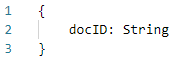
\includegraphics{img/getdocumentbyid1.PNG}
    \caption{getDocumentByID Received Data Format}
    \label{fig:getdocumentbyid1}
\end{figure}
\textbf{Returned Data}:
\newline
\newline
This endpoint will return two possible JSON documents depending on the success of the query. To avoid errors, the API will check if the ID provided is both a valid ObjectID and if the query actually returned some document data. If neither of those checks pass, the API will return a JSON document in the format found in Figure \ref{fig:getdocumentbyid3}.
\begin{figure}[H]
    \centering
    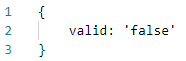
\includegraphics{img/getdocumentbyid3.PNG}
    \caption{getDocumentByID Returned Data Format}
    \label{fig:getdocumentbyid3}
\end{figure}
Otherwise, a successful query will return a variable JSON document that holds only the raw document data found by the query. This is essentially plucking a document out of the database without any modifications to it's structure An example of what this JSON document looks like can be found in Figure \ref{fig:getdocumentbyid2}.

\begin{figure}[H]
    \centering
    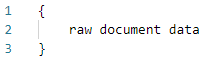
\includegraphics{img/getdocumentbyid2.PNG}
    \caption{getDocumentByID Returned Data Format}
    \label{fig:getdocumentbyid2}
\end{figure}
